% Die vorangehenden fachlichen Kapitel 2 und 3 sind im aktuellen Template noch nicht angelegt.
% Der Zähler stellt vorläufig die vorgegebene Kapitelnummer her und ist nach der Integration der Kapitel 2 und 3 zu entfernen.
\setcounter{section}{3}
\section{Konzeption des IFC-basierten Annotationsmodells}\label{sec:ifc-annotationsmodell}
\subsection{Modellierungsziele und zentrale Designentscheidungen}\label{subsec:modellierungsziele-annotationsmodell}
Gebäudemodelle im IFC-Format beschreiben ein Bauwerk als strukturierte Menge von Objekten mit
Eigenschaften, Beziehungen und geometrischer Repräsentation. Sie enthalten damit einen erheblichen
Teil der Informationen, die ein mobiler Roboter über seine Einsatzumgebung benötigt, jedoch keine
Beschreibung dessen, was in dieser Umgebung geschehen soll. Robotische Systeme wiederum operieren
mit Aktionen, Zuständen und Posen, verfügen aber in der Regel über keine semantisch strukturierte
Verbindung zu den Bauteilen, auf die sich diese Aktionen beziehen. Das in dieser Arbeit entwickelte
Annotationsmodell setzt an dieser Lücke an. Sein übergeordnetes Ziel besteht darin, Robotermissionen
so zu beschreiben, dass sie eindeutig auf Objekte des Gebäudemodells bezogen sind, über die Laufzeit
einer einzelnen Editor-Sitzung hinaus Bestand haben und sowohl in die IFC-Datei hinein als auch aus
ihr wieder heraus verarbeitet werden können. Aus dieser Zielsetzung leiten sich die im Folgenden
dargestellten Modellierungsziele und die daraus resultierenden grundlegenden Entwurfsprinzipien ab.

Das erste Modellierungsziel betrifft die strukturierte Repräsentation der Aufgabenbeschreibung
selbst. Eine Robotermission ist keine einzelne Handlung, sondern eine Menge ausführbarer Aufgaben,
die inhaltlich zusammengehören und in einer bestimmten Reihenfolge abgearbeitet werden. Das Modell
trennt deshalb konsequent zwischen der Mission als übergeordneter, fachlich benannter Einheit und
den einzelnen Aufgaben, die den tatsächlich ausführbaren Handlungen entsprechen. Wesentlich ist
dabei eine zweite Trennung innerhalb der Mission: Die Zugehörigkeit einer Aufgabe zu einer Mission
und ihre Anzeigereihenfolge sind nicht dasselbe wie ihre Ausführungsabhängigkeit von einer anderen
Aufgabe. Im Domänenmodell ist diese Unterscheidung nicht nur konventionell festgelegt, sondern
strukturell erzwungen: Die Mission führt die Zugehörigkeit über ein eigenes Feld ihrer
Aufgabenliste, während Ausführungsabhängigkeiten in einer davon unabhängigen Liste eigenständiger
Abhängigkeitsobjekte geführt werden. Diese Trennung verhindert, dass eine rein hierarchische oder
darstellungsbedingte Ordnung fälschlich als zeitliche Aussage interpretiert wird, und sie schafft
die Voraussetzung dafür, später auch nichtlineare Abläufe zu beschreiben, ohne die Modellstruktur zu
verändern. Die konkrete Ausprägung dieser Konzepte als RobotMission, RobotTask und RobotTaskSequence
wird in Kapitel 4.2 behandelt.

Das zweite Modellierungsziel ist die explizite Verknüpfung von Aufgaben mit Elementen des
Gebäudemodells. Eine Aufgabe wie das Öffnen einer Tür oder das Betätigen eines Schalters ist ohne
Objektbezug nicht ausführbar; der Bezug ist damit kein optionales Zusatzattribut, sondern ein
konstitutiver Bestandteil der Aufgabenbeschreibung. Daraus folgt unmittelbar die Anforderung nach
einer möglichst stabilen Objektidentität. Der Editor stellt Gebäudemodelle nicht unmittelbar aus der
IFC-Datei dar, sondern über eine performante Darstellungsstruktur, deren interne Kennungen an die
jeweilige Sitzung, das jeweilige Laufzeitmodell und den jeweiligen Ladevorgang gebunden sind. Eine
Annotation, die sich auf solche Kennungen stützt, verliert ihre Bedeutung, sobald das Modell erneut
geladen, in einem anderen Werkzeug geöffnet oder in geänderter Form weitergegeben wird. Das
Domänenmodell begegnet dieser Anforderung nicht nur durch Konvention, sondern durch die Typstruktur
des Objektbezugs selbst: Eine gültige Referenz besitzt entweder eine dauerhafte IFC-GlobalId,
optional ergänzt um eine lokale Kennung zur effizienten Laufzeitauflösung, oder sie besitzt zwingend
sowohl eine modelllokale Kennung als auch eine Kennung des zugehörigen Laufzeitmodells, wenn keine
GlobalId vorliegt. Der modelllokale Rückfallweg ist damit nur innerhalb genau des Quellmodells
auflösbar, dem er zugeordnet ist. Die technischen Konsequenzen dieser Festlegung, insbesondere das
Verhalten bei fehlenden oder mehrdeutigen Referenzen, werden in Kapitel 4.4 behandelt.

Eng damit verbunden ist das dritte und für die fachliche Qualität des Modells zentrale Ziel: die
Trennung zwischen dem Gebäudeobjekt und der Roboteraktion. Eine Tür ist ein Bauteil mit statischen
Eigenschaften; dass ein Roboter sie in einer bestimmten Aufgabe öffnen soll, ist demgegenüber eine
Aussage über diese Aufgabe und nicht über die Tür. Das Modell hinterlegt die konkrete
Aktionssemantik daher ausschließlich an der Aufgabe und niemals am referenzierten Bauteil. Die Tür
wird durch die Annotation nicht zu einer „OPEN-Tür“; sie bleibt eine Tür, auf die sich
unterschiedliche Aufgaben mit unterschiedlichen Aktionen beziehen können. Diese Trennung ist im
Prototyp doppelt abgesichert: Der Typ des Objektbezugs sieht kein Feld für Aktionsdaten vor, und die
Validierung weist eine Aufgabenreferenz, die dennoch aktionsartige Eigenschaften trägt – etwa einen
Zielzustand oder eine geforderte Fähigkeit –, ausdrücklich als Fehler zurück. Diese doppelte
Absicherung ist Voraussetzung dafür, dass dasselbe Gebäudemodell für mehrere, voneinander
unabhängige Missionen wiederverwendbar bleibt und dass dieselbe Tür innerhalb einer Mission zunächst
geöffnet und später wieder geschlossen werden kann, ohne dass sich ihre Eigenschaften
widersprüchlich verändern. Eine Vorannotation grundsätzlich möglicher Interaktionen am Gebäudeobjekt
selbst – also die Aussage, welche Aktionen ein Objekt prinzipiell zuließe – ist im aktuellen Stand
nicht implementiert und stellt eine mögliche Erweiterung dar; sie würde die hier beschriebene
Trennung ergänzen, nicht aufheben.

Das vierte Modellierungsziel verallgemeinert diesen Gedanken zu einer Trennung von Ebenen, wie sie
Abbildung~\ref{fig:trennung-der-ebenen} zusammenfasst.

\begin{figure}[htbp]
    \centering
    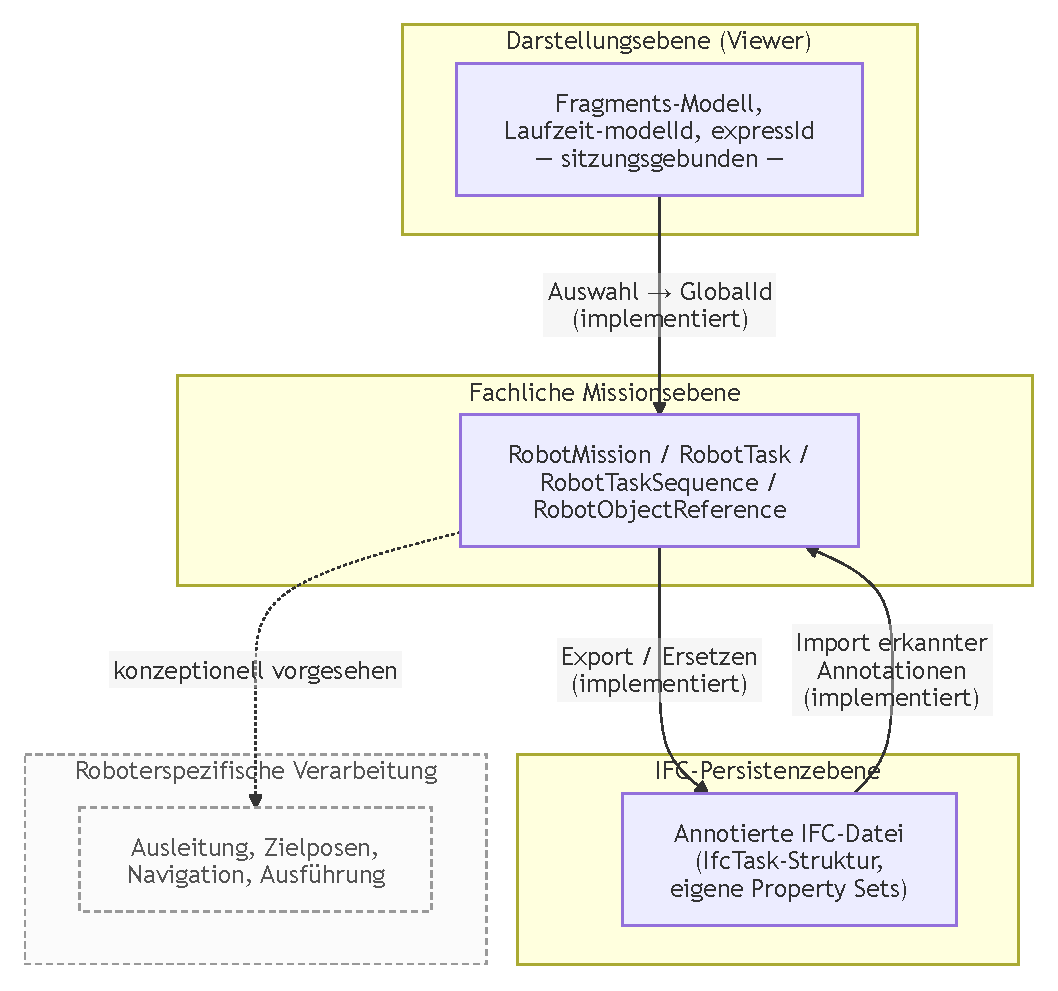
\includegraphics[width=0.4\textwidth]{pics/abbildung_4-1_trennung_der_ebenen.pdf}
    \caption{Trennung der Ebenen}
    \label{fig:trennung-der-ebenen}
\end{figure}

Zu unterscheiden sind das fachliche Missions- und Aufgabenmodell, die
IFC-Repräsentation dieses Modells und die Darstellungsstruktur des Viewers. Das fachliche Modell ist
als eigenständige Schicht ausgeführt, die weder von der verwendeten 3D-Bibliothek noch von den
Kennungen der Darstellungsstruktur, vom Browser-Speicher oder von der konkreten STEP-Syntax abhängt.
Der Übersetzungsschritt in IFC-nahe Strukturen ist als eigene, von der eigentlichen
Dateimanipulation getrennte Schicht realisiert: Ein reiner Mapper erzeugt aus einer gültigen Mission
ausschließlich typisierte Zwischenrecords und bricht bereits vor der Erzeugung eines einzigen
Records ab, wenn die Mission blockierende Validierungsfehler enthält. Er verändert keine IFC-Datei,
lädt keine WASM-Laufzeit und enthält keine Viewer-Logik. Das daraus abgeleitete Modellierungsziel
lautet, dass Robotermissionsdaten nicht von temporären Rendering-Strukturen oder viewer-spezifischen
Kennungen abhängig sein dürfen. Die technische Ausgestaltung dieser Schichtung ist Gegenstand des
Implementierungskapitels; für die Modellkonzeption ist allein maßgeblich, dass die fachliche Aussage
einer Annotation unabhängig von der Art ihrer Darstellung gültig bleibt.

Das fünfte Ziel betrifft IFC als Träger der Annotation in beide Richtungen. Missionsinformationen
sollen so weit sinnvoll in der IFC-Struktur selbst abgebildet werden, dass Gebäudeinformation und
Missionsbezug gemeinsam transportiert werden können und keine zweite, separat zu pflegende
Hauptdatenquelle entsteht. Im Prototyp ist dazu nicht nur der Export einer Mission in die zugrunde
liegende IFC-Quelldatei umgesetzt, sondern auch das umgekehrte Wiedereinlesen: Vom System selbst
erzeugte, projekteigene Missionsannotationen werden beim Laden einer IFC-Datei erkannt und zu
RobotMission- und RobotTask-Aggregaten rekonstruiert. Eine importierte Mission kann im Editor
verändert und anschließend erneut exportiert werden, wobei der zuvor erkannte Missionsgraph gezielt
ersetzt statt bei jedem Durchlauf neu angehängt wird; nach dem Export wird die erzeugte Datei zur
Absicherung erneut geöffnet, die Mission erneut importiert und mit dem beabsichtigten Domänenmodell
semantisch verglichen, bevor die neuen Bytes als Ausgangspunkt für den nächsten Zyklus übernommen
werden. Für deterministisch wiedererkennbare Missionsentitäten bleiben bestehende IFC-GlobalIds über
solche Zyklen hinweg erhalten; bestehende Building-GlobalIds werden dabei nicht angetastet. Dennoch
ist eine Abgrenzung notwendig: Der implementierte Roundtrip bezieht sich ausschließlich auf den vom
System erkannten, projekteigenen Missionsgraphen. Strukturelle Änderungen am Gebäudemodell selbst
werden nicht zurückgeschrieben, Modelle ohne erhaltene IFC-Quelle sind nicht exportierbar, und nicht
jedes IFC-Schema wird vom Missionswriter unterstützt. Ein verlustfreier Roundtrip beliebiger
Modelländerungen ist damit ausdrücklich nicht Bestandteil des Prototyps.

Aus dem Anspruch, das Modell über den Prototyp hinaus verwendbar zu halten, folgt als sechstes Ziel
die Erweiterbarkeit. Zusätzliche Aktionsarten, weitere Aufgabeneigenschaften, differenziertere
Objektrollen, weitere zeitliche Beziehungsarten und roboterspezifische Ausleitungen sollen ergänzt
werden können, ohne die Grundstruktur neu entwerfen zu müssen. Getragen wird dies durch mehrere im
Code erkennbare Entscheidungen: Die Aktionssemantik liegt in einem klar abgegrenzten, überwiegend
optional besetzten Eigenschaftsbereich der Aufgabe; Objektrollen werden über benannte Relationen und
nicht über strukturell verschiedene Modellelemente unterschieden; und die Annotation trägt mit einer
eigenen Konstante eine explizite Schemaversion, die in jede exportierte Mission geschrieben wird,
sodass ältere Annotationsstände beim Einlesen erkennbar und behandelbar bleiben.

Als siebtes Ziel ist die Validierbarkeit zu nennen. Eine Annotation, die sowohl exportiert als auch
wieder importiert werden soll, muss vor der Weitergabe überprüfbar sein. Der Prototyp unterscheidet
dabei durchgängig zwischen blockierenden Fehlern und nicht blockierenden Warnungen: Unvollständige
Entwürfe bleiben bearbeitbar, während sowohl die Abbildung in IFC-nahe Records als auch der
tatsächliche Export nur für Missionen zugelassen werden, die vollständig gültig sind und deren
Objektbezüge im gewählten Quellmodell eindeutig aufgelöst werden können. Fehlende Typinformationen
des referenzierten Bauteils führen zu einer Warnung statt zu einer Zurückweisung einer ansonsten
plausiblen Aufgabe; ein bekannter, aber unpassender Objekttyp führt dagegen zu einem blockierenden
Fehler.

Die Frage der Interoperabilität ist demgegenüber differenziert zu beantworten. Das Modell verwendet
für Struktur und Beziehungen reguläre IFC-Entitäten, sodass eine annotierte Datei syntaktisch gültig
bleibt und die Missionsstruktur von generischen Werkzeugen als Prozessstruktur gelesen werden kann.
Die eigentliche Robotiksemantik – die Aktionswerte und die Bedeutung der eigenen Eigenschaftsgruppen
– ist hingegen projektspezifisch und nicht Bestandteil des IFC-Standards. Daraus folgt, dass die
strukturelle Lesbarkeit durch Fremdsysteme angenommen werden kann, die inhaltliche Interpretation
der Robotiksemantik durch Fremdsysteme jedoch nicht. Ein Nachweis der tatsächlichen Interpretation
durch andere Werkzeuge wurde im Rahmen dieser Arbeit nicht geführt; die Grenzen dieser
Interoperabilität werden in Abschnitt 4.12 gesondert diskutiert.

Schließlich soll das Annotationsmodell die fachliche Grundlage für eine spätere Verarbeitungskette
bilden, die von der IFC-Annotation über das interne Missionsmodell zu einer roboterspezifischen
Ausleitung, zu Zielposen und Navigationsdaten und letztlich zur Ausführung führt. Von dieser Kette
ist im vorliegenden Stand der vordere, bidirektionale Teil – Export, Import und verifizierter
Roundtrip – umgesetzt; die roboterspezifische Weiterverarbeitung ist konzeptionell vorgesehen und
wird in Kapitel 7 behandelt. Für die Modellierung ist dieser Ausblick dennoch bedeutsam, weil er
begründet, weshalb Aktionsart, Objektbezug, Objektrolle und Reihenfolge explizit und getrennt
voneinander repräsentiert werden müssen: Erst diese Explizitheit erlaubt es, aus einer Annotation
später eine ausführbare Anweisung abzuleiten, ohne fachliche Annahmen aus einer Darstellungsform
rekonstruieren zu müssen. Abbildung~\ref{fig:grundstruktur_annotationsmodell} fasst die daraus resultierende Grundstruktur zusammen.
\begin{figure}[htbp]
    \centering
    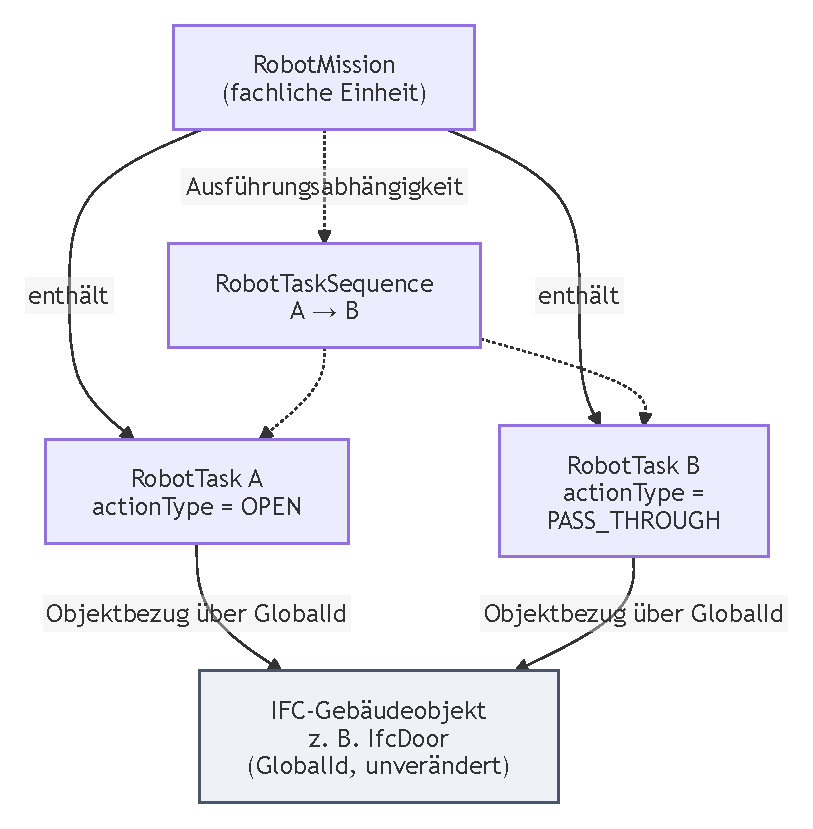
\includegraphics[width=0.4\textwidth]{pics/abbildung_4-2_grundstruktur_annotationsmodell.pdf}
    \caption{Grundstruktur Annotationsmodell}
    \label{fig:grundstruktur_annotationsmodell}
\end{figure}


Die in diesem Abschnitt formulierten Ziele bleiben zunächst Anforderungen an das Datenmodell. Wie
sie durch ein konkretes internes Domänenmodell mit Missionen, Aufgaben, Sequenzen, Objektbezügen und
Aktionsparametern eingelöst werden, ist Gegenstand des folgenden Abschnitts 4.2.

\subsection{Internes Domänenmodell}\label{subsec:Internes_Domänenmodell}
Aus den zuvor formulierten Modellierungszielen wird im Folgenden das interne Domänenmodell
abgeleitet. Während Kapitel 4.1 begründet hat, *welche* fachlichen Sachverhalte überhaupt
repräsentiert werden müssen, beschreibt dieses Unterkapitel, *wie* diese Sachverhalte innerhalb des
Editors als typisierte Datenstruktur ausgedrückt werden. Leitend ist dabei die Frage, wie
Robotermissionen unabhängig von IFC-Serialisierung, Viewer und Benutzeroberfläche fachlich
repräsentiert werden können.

Das Domänenmodell bildet die fachliche Zwischenschicht des Systems. Es ist im Prototyp als
eigenständige Modulgruppe unter `src/domain/robot-tasks/` umgesetzt und umfasst die Typdefinitionen
(`types.ts`), die Erzeugungs- und Änderungsoperationen (`builders.ts`), die Sequenzlogik
(`sequencing.ts`) sowie die Validierung (`validation.ts`). Dieser Zuschnitt ist bewusst gewählt:
Weder die dreidimensionale Darstellung eines Gebäudemodells noch die konkrete IFC-Syntax sollen
bestimmen, wie eine Mission fachlich beschrieben wird. Das Domänenmodell ist damit nicht ein
technisches Zwischenformat, sondern die maßgebliche fachliche Beschreibung, aus der sowohl die
Darstellung im Editor als auch die spätere IFC-Repräsentation abgeleitet werden.
Abbildung~\ref{fig:grundstruktur_domaenenmodell} zeigt die Struktur des Modells im Überblick.

\begin{figure}[htbp]
    \centering
    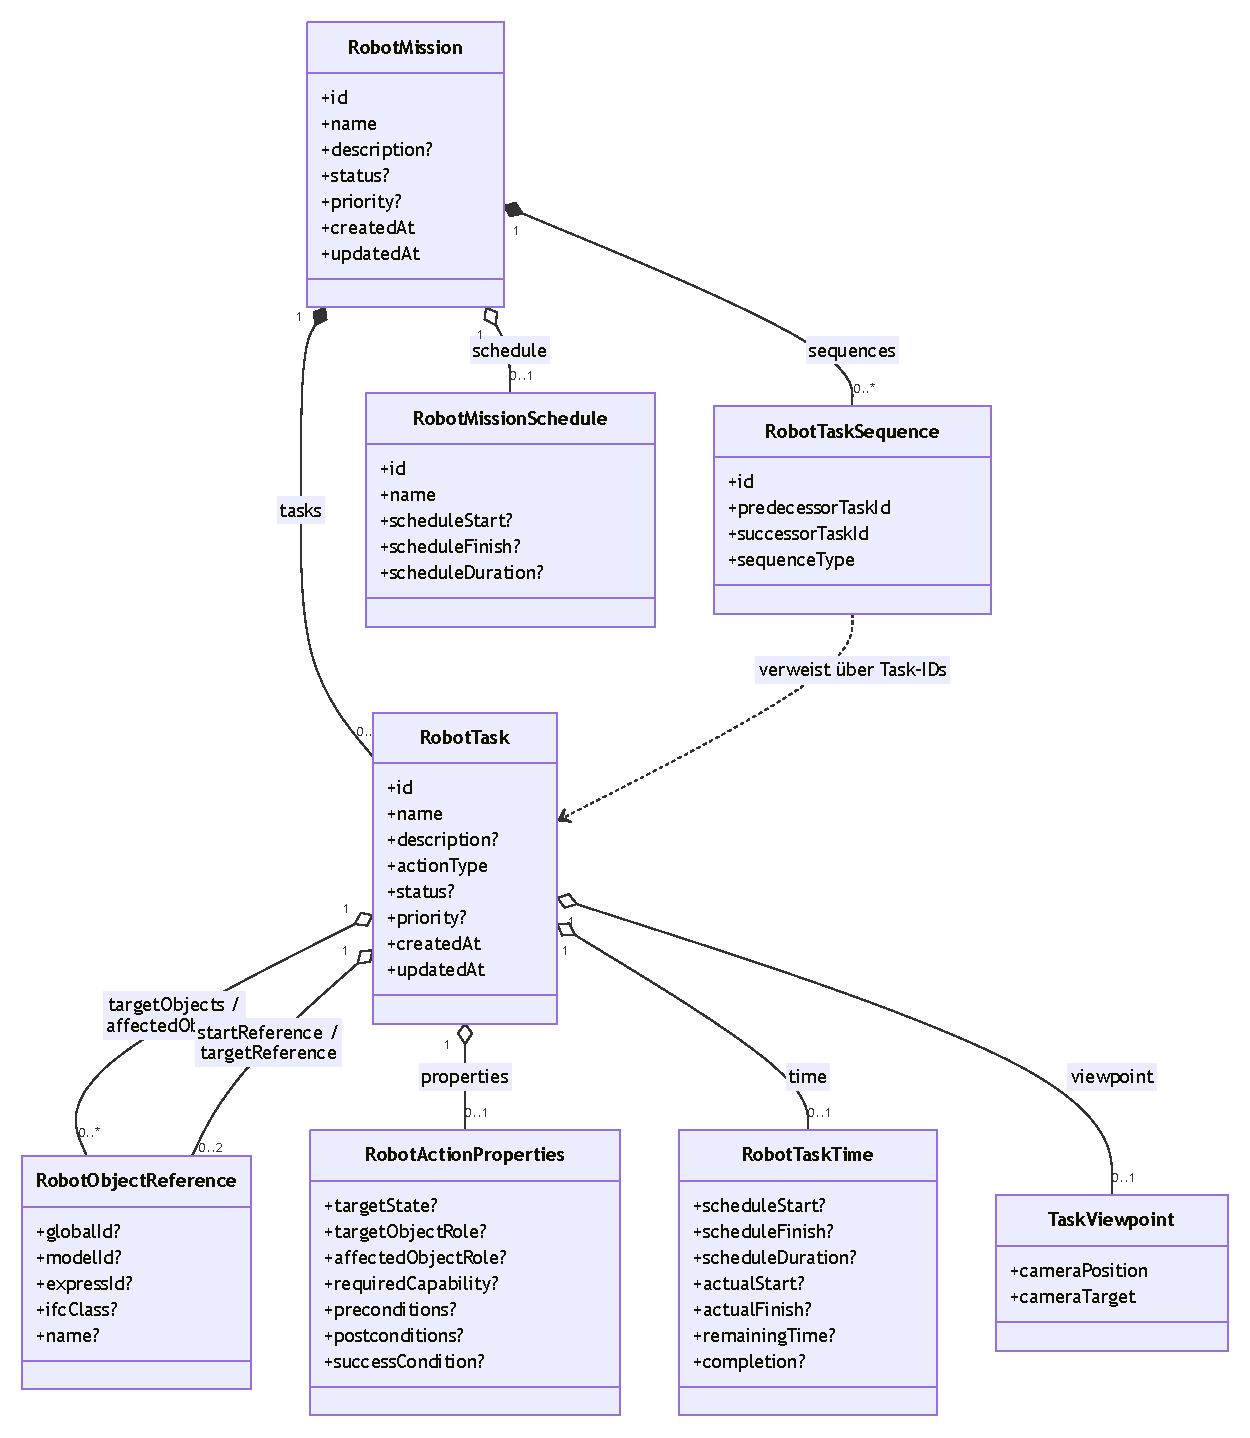
\includegraphics[width=0.7\textwidth]{pics/struktur_internes_domänenmodell.pdf}
    \caption{Struktur des internen Domänenmodells}
    \label{fig:grundstruktur_domaenenmodell}
\end{figure}
\subsubsection{Die Mission als übergeordnete Einheit}\label{Mission_Einheit}
`RobotMission` bezeichnet eine vollständige Robotermission und bildet die übergeordnete Einheit des
Modells, also diejenige Struktur, über die alle zugehörigen Informationen erreichbar sind und deren
Konsistenz als Ganzes geprüft werden kann. In der Architekturdokumentation des Prototyps wird sie
als Aggregat-Root bezeichnet; fachlich entscheidend ist, dass ausführbare Schritte, deren
Abhängigkeiten und die optionale Zeitplanung nicht unabhängig voneinander existieren, sondern stets
im Kontext genau einer Mission.

Eine Mission trägt eine stabile anwendungsseitige Kennung (`id`), einen menschenlesbaren Namen sowie
eine optionale Beschreibung. Die Kennung ist ausdrücklich eine Anwendungs-ID und keine
IFC-Identität; die Frage, wie beide Identitätsräume beim Export und Import aufeinander abgebildet
werden, wird erst in Kapitel 4.4 und Kapitel 4.9 behandelt. Ergänzend führt die Mission einen
aggregierenden Bearbeitungsstatus und eine Priorität. Bemerkenswert ist, dass Status und Priorität
im Modell durch dieselben Typen beschrieben werden wie auf Task-Ebene; Mission und Task teilen damit
dasselbe Vokabular für Lebenszyklus und Dringlichkeit, was den Aufbau der Bearbeitungsoberfläche
vereinheitlicht.

Die eigentliche fachliche Substanz liegt in drei Feldern. `tasks` enthält die ausführbaren
Einzelschritte der Mission, `sequences` die expliziten gerichteten Abhängigkeiten zwischen diesen
Schritten, und `schedule` optional eine Zeitplanung der Mission als Ganzes. Hinzu kommen ein
Erstellungs- und ein Änderungszeitstempel, die nachvollziehbar machen, wann eine Mission zuletzt
bearbeitet wurde. Wesentlich ist, dass die Mission selbst keine Roboteraktion beschreibt: Sie ist
Container und Klammer, nicht ausführbare Handlung. Jede konkrete Tätigkeit wird ausschließlich durch
die enthaltenen Tasks ausgedrückt.

\subsubsection{Der Task als ausführbare Einheit}\label{Task_Einheit}
`RobotTask` bezeichnet einen ausführbaren Einzelschritt innerhalb einer Mission. Der Task ist die
zentrale Struktur des Modells, weil er unterschiedliche Informationsbereiche zusammenführt, die im
Modell dennoch klar getrennt bleiben.

Den fachlichen Kern bildet die Aktion: Jeder Task besitzt neben Kennung, Name und optionaler
Beschreibung genau einen `actionType`, also die konkrete auszuführende Roboteraktion. Der zweite
Bereich umfasst die Bezüge zu Gebäudeelementen. Hier unterscheidet das Modell zwischen
`targetObjects` als unmittelbar adressierten oder als Kontext genutzten Objekten und
`affectedObjects` als indirekt betroffenen Objekten; für Bewegungsaufgaben treten zusätzlich
`startReference` und `targetReference` als Ausgangs- und Zielbezug hinzu. Der dritte Bereich sind
die Aktionsparameter (`properties`), der vierte die zeitlichen Informationen (`time`). Als fünfter,
optionaler Bereich können mit `viewpoint` und `markerPosition` annotationsbezogene
Zusatzinformationen hinterlegt werden, die den Task im Viewer wiederauffindbar machen. Abgeschlossen
wird die Struktur durch Status, Priorität und Zeitstempel.

Abstrahiert ergibt sich damit folgender Aufbau:
\begin{figure}[htbp]
    \centering
    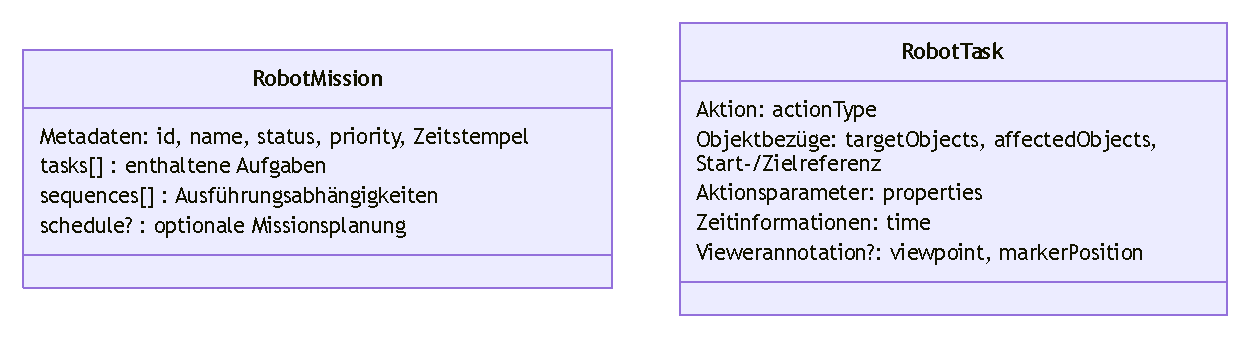
\includegraphics[width=0.4\textwidth]{pics/Attributstruktur.pdf}
    \caption{Attributstruktur RobotMission und RobotTask}
    \label{fig:Attributstruktur}
\end{figure}

Die Trennung dieser Bereiche ist keine bloße Ordnungsfrage. Sie erlaubt es, denselben Task
schrittweise anzureichern – zunächst Aktion und Zielobjekt, später Parameter und Zeitplanung –, ohne
dass unvollständige Zwischenstände strukturell unzulässig wären. Zugleich stellt sie sicher, dass
die einzelnen Bereiche später auf unterschiedliche IFC-Konstrukte abgebildet werden können, ohne im
Domänenmodell vermischt zu sein.

\subsubsection{Referenzen und ergänzende Wertobjekte}\label{Ref_Ojekte}
`RobotObjectReference` bezeichnet den fachlichen Verweis auf ein IFC-Objekt. Entscheidend ist, dass
im Domänenmodell keine Viewer- oder Three.js-Objekte, keine Geometrie und keine Rendering-Handles
gespeichert werden, sondern ausschließlich eine schlanke Identitätsbeschreibung. Bevorzugt wird die
`globalId`, also die dauerhafte IFC-Objektidentität. Steht diese nicht zur Verfügung, ist ein
modelllokaler Fallback aus `modelId` und `expressId` zulässig; die Typdefinition erzwingt dabei
bereits auf Typebene, dass eine `expressId` ohne `globalId` nur zusammen mit der zugehörigen
`modelId` verwendet werden kann, da Express-IDs nur innerhalb einer Modellserialisierung eindeutig
sind. Ergänzend können mit `ifcClass` und `name` beschreibende Angaben zum Objekt geführt werden.
Die vollständige Referenzierungsstrategie einschließlich ihrer Konsequenzen für Modellgrenzen und
wiederholte Serialisierungen ist Gegenstand von Kapitel 4.4.

Wesentlich für das Verständnis des Modells ist, dass die Referenz bewusst frei von Aktionssemantik
bleibt. Sie beantwortet die Frage, *welches* Bauteil gemeint ist, nicht die Frage, *was* mit ihm
geschehen soll. Diese zweite Frage beantwortet `RobotActionProperties`, also die strukturierte
Beschreibung der konkreten Aktionsanforderung eines Tasks. Dort können unter anderem ein
angestrebter Zielzustand, die semantischen Rollen der adressierten und der betroffenen Objekte, eine
erforderliche Roboterfähigkeit sowie Vor-, Nachbedingungen und ein Erfolgskriterium hinterlegt
werden. Da diese Angaben am Task und nicht am Objekt hängen, kann dasselbe IFC-Objekt in
verschiedenen Tasks mit unterschiedlichen Anforderungen verwendet werden – etwa eine Tür, die in
einem Schritt geöffnet und in einem späteren wieder geschlossen wird. Die Bedeutung der einzelnen
Aktionsarten wird in Kapitel 4.3 behandelt.

`RobotTaskTime` bezeichnet die zeitliche Beschreibung eines einzelnen Tasks und umfasst geplanten
Start, geplantes Ende und geplante Dauer, den tatsächlichen Start und das tatsächliche Ende, die
verbleibende Dauer sowie einen Fertigstellungsgrad. Diese Angaben sind bewusst nicht Teil von
`RobotActionProperties`, obwohl beide Strukturen den Task ergänzen. Aktionsparameter beschreiben die
fachliche Anforderung an die Ausführung und sind projektspezifisch; Zeitangaben beschreiben dagegen
Planung und Fortschritt und entsprechen einem in IFC bereits vorhandenen Konzept, das in Kapitel 4.8
aufgegriffen wird. Die Trennung im Domänenmodell nimmt diese unterschiedliche Herkunft vorweg und
vermeidet, dass Planungsdaten in einer projekteigenen Parameterstruktur verborgen werden.

Auf Missionsebene existiert mit `RobotMissionSchedule` eine optionale Zeitplanung für die Mission
als Ganzes, bestehend aus Kennung, Name sowie geplantem Start, Ende und Dauer. Sie ersetzt die
Task-Zeiten nicht, sondern beschreibt einen übergeordneten Rahmen: Der Task-Zeitbereich betrifft die
Ausführung eines einzelnen Schritts einschließlich des tatsächlichen Verlaufs, die Missionsplanung
dagegen ausschließlich die geplante zeitliche Einordnung des Gesamtvorgangs.

\subsubsection{Hierarchie und Ausführungsabhängigkeit als getrennte Strukturen}
`RobotTaskSequence` bezeichnet eine eigenständige gerichtete Abhängigkeit zwischen zwei Tasks. Eine
Sequenz besitzt eine eigene stabile Kennung, verweist über Task-IDs auf einen Vorgänger und einen
Nachfolger und trägt einen Sequenztyp, der die Art der zeitlichen Beziehung angibt. Sequenzen sind
damit eigenständige Elemente der Mission und keine Eigenschaft eines Tasks.

Daraus ergibt sich die für dieses Kapitel zentrale Unterscheidung: `RobotMission.tasks` beschreibt,
welche ausführbaren Schritte zur Mission gehören, und legt zugleich deren deterministische
Darstellungs- und Hierarchieordnung fest. `RobotMission.sequences` beschreibt demgegenüber, welche
zeitlichen Abhängigkeiten zwischen diesen Schritten bestehen. Beide Strukturen ließen sich nicht
ohne Informationsverlust durch ein einziges sortiertes Task-Array ersetzen. Ein Array kann
ausschließlich eine lineare Folge ausdrücken; ein Abhängigkeitsgraph kann darüber hinaus unabhängige
Zweige und mehrere Vorgänger desselben Nachfolgers darstellen. Zwei Tasks, die in beliebiger
Reihenfolge oder parallel ausgeführt werden dürfen, sind in einem Array zwangsläufig geordnet, im
Graphen dagegen korrekt als unabhängig beschreibbar.
Abbildung~\ref{fig:Missionsstruktur_ausführung} stellt beide Sichten einander gegenüber.
\begin{figure}[htbp]
    \centering
    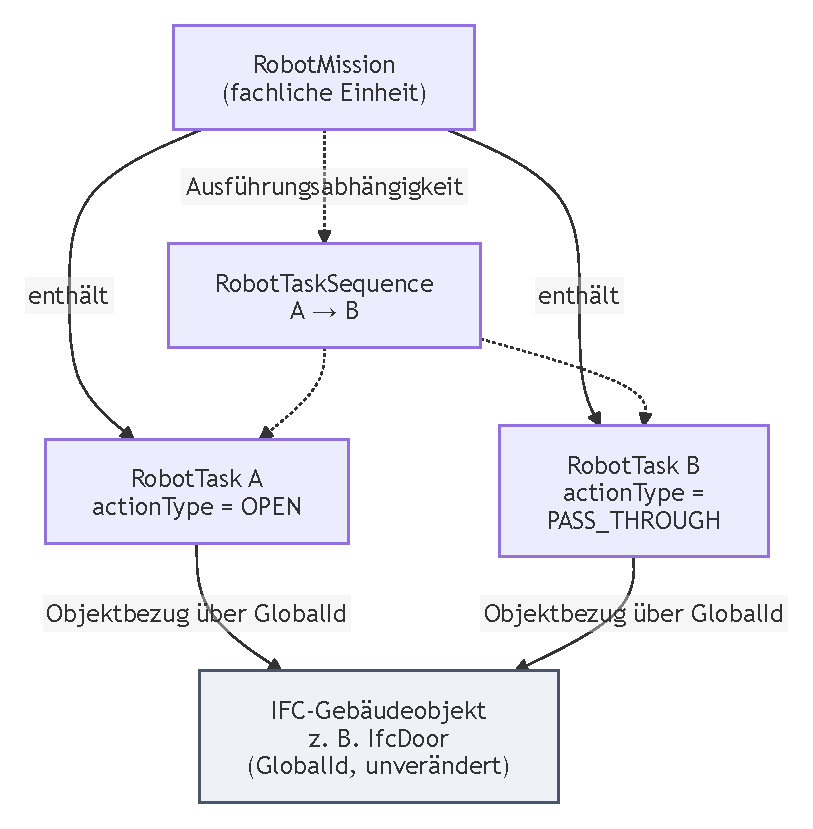
\includegraphics[width=0.7\textwidth]{pics/Missionsstruktur.pdf}
    \caption{Gegenüberstellung der Missionsstruktur und der Ausführungsabhängigkeiten}
    \label{fig:Missionsstruktur_ausführung}
\end{figure}

Die Implementierung behandelt beide Strukturen konsequent getrennt. Die Sequenzlogik prüft den
Graphen auf Selbstbezüge, auf Verweise auf unbekannte Tasks und auf Zyklen und kann aus Hierarchie
und Sequenzen eine ausführungsgerechte Reihenfolge ableiten, wobei die Hierarchieordnung als
deterministisches Tie-Breaking-Kriterium für voneinander unabhängige Tasks dient. Legt eine
Anwenderin oder ein Anwender eine rein lineare Reihenfolge fest, wird daraus eine vollständige Kette
vom Typ `FINISH_START` erzeugt; auch dieser Fall wird jedoch als Sequenzgraph gespeichert und nicht
auf die Array-Reihenfolge reduziert. Die inhaltliche Semantik der Sequenztypen sowie die
Zyklusbehandlung im Detail sind Gegenstand von Kapitel 4.5.

\subsubsection{Domänenoperationen und Invarianten}
Damit das Modell nicht nur beschreibend, sondern auch verlässlich ist, werden Domänenobjekte nicht
frei zusammengesetzt, sondern über dedizierte Erzeugungs- und Änderungsoperationen gebildet.
Missionen und Tasks entstehen über eigene Erzeugungsfunktionen, weitere Operationen fügen einer
Mission Tasks hinzu, weisen Ziel- und betroffene Objekte zu, setzen Start- und Zielbezug einer
Bewegungsaufgabe, ersetzen die Aktionsparameter oder die Zeitangaben eines Tasks.

Vier Eigenschaften dieser Operationen prägen das Modell. Erstens werden Eingaben normalisiert:
Pflichttexte wie Kennungen und Namen werden bereinigt, und eine leere Angabe führt unmittelbar zu
einem Domänenfehler statt zu einem strukturell gültigen, fachlich aber unbrauchbaren Objekt.
Zweitens erzeugt jede Änderung eine neue Objektstruktur, statt bestehende Objekte zu verändern;
Missionen und Tasks werden also als unveränderliche Werte behandelt, was Vergleiche zwischen einem
beabsichtigten und einem rekonstruierten Zustand erst zuverlässig möglich macht. Drittens werden
Eindeutigkeitsregeln früh durchgesetzt: Task-Kennungen müssen innerhalb einer Mission eindeutig
sein, weil Sequenzen genau über diese Kennungen auflösen, und dieselbe Objektidentität wird einem
Task nicht mehrfach zugewiesen. Viertens wird bei jeder Änderung der Änderungszeitpunkt
fortgeschrieben.

Ergänzend prüft eine eigene Validierung die fachlichen Invarianten des Modells und meldet
blockierende Fehler und nicht blockierende Warnungen als maschinen- und menschenlesbare Befunde. Für
dieses Kapitel ist vor allem bemerkenswert, dass die Validierung die Trennung von Objekt und Aktion
ausdrücklich absichert: Aktionsparameter, die an einer Objektreferenz statt am Task hinterlegt
wurden – etwa aus deserialisierten Fremddaten –, werden als Verstoß gemeldet. Die vollständigen
Regeln werden in Kapitel 4.10 dargestellt.

\subsubsection{Frameworkunabhängigkeit und gemeinsame Repräsentation im Roundtrip}
Die Domänenschicht des Prototyps ist frei von direkten Abhängigkeiten zu Three.js, That Open
Components, Fragments, `web-ifc`, Browser-Oberfläche und Browser-Persistenz; ihre Module verweisen
ausschließlich aufeinander. Die Abhängigkeitsrichtung verläuft ausnahmslos von den äußeren Schichten
zur Domäne: Anwendungsdienste, Persistenzadapter, Viewer-Adapter, IFC-Mapping sowie Import- und
Exportmodule beziehen ihre Typen und Operationen aus der Domäne, während umgekehrt keine dieser
Technologien in die Domäne gelangt. Der Viewer-Adapter etwa übersetzt eine Auswahl im
dreidimensionalen Modell in eine `RobotObjectReference`; die Domäne kennt anschließend nur noch
diese Referenz und nicht mehr das Auswahlobjekt, aus dem sie entstanden ist. Fachlich bedeutet dies,
dass die Frage, wie eine Mission beschrieben wird, unabhängig davon beantwortet wird, wie sie
dargestellt, gespeichert oder serialisiert wird:

\begin{figure}[htbp]
    \centering
    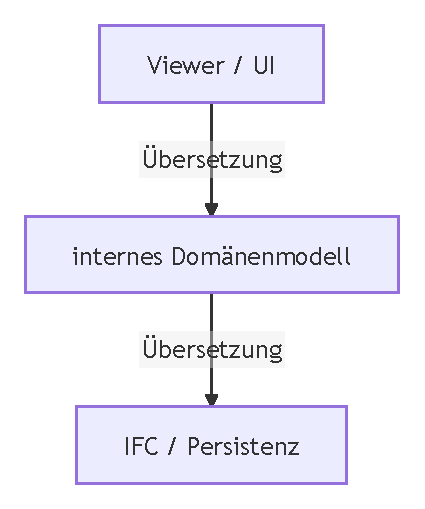
\includegraphics[width=0.4\textwidth]{pics/Schichten_pipeline.pdf}
    \caption{Pipeline}
    \label{fig:Pipeline}
\end{figure}

Die technische Umsetzung dieser Schichtung ist Gegenstand von Kapitel 5.1; für das Datenmodell
selbst ist entscheidend, dass Auswahlmechanismen, Renderingstrukturen und Dateiformate keinen
Eingang in die fachliche Beschreibung finden.

Diese Unabhängigkeit ist zugleich die Voraussetzung dafür, dass das Modell im implementierten
IFC-Roundtrip als gemeinsamer Bezugspunkt dienen kann. Neu erstellte Missionen, aus einer
annotierten IFC-Datei rekonstruierte Missionen, im Editor bearbeitete Missionen und erneut zu
exportierende Missionen werden durch dieselben Typen beschrieben. Beide Richtungen des Austauschs
greifen dabei nicht nur auf dieselben Typen, sondern auch auf dieselbe Domänenvalidierung zurück:
Sowohl die Rekonstruktion einer Mission aus IFC als auch die Abbildung einer Mission auf IFC-nahe
Strukturen prüfen das Ergebnis gegen die fachlichen Invarianten des Domänenmodells. Konzeptionell
gilt damit: IFC-Import und IFC-Export treffen sich im selben internen Domänenmodell. Dass
dieselbe Struktur beide Richtungen bedient, ist auch der Grund dafür, dass Hierarchie und Sequenzen
getrennt geführt werden – nur so bleiben beide Informationen beim Rücklesen unterscheidbar. Die
Implementierung von Import, Replacement-Export und semantischem Vergleich wird in Kapitel 5.9
beziehungsweise in der Evaluation behandelt.
